
%(BEGIN_QUESTION)
% Copyright 2012, Tony R. Kuphaldt, released under the Creative Commons Attribution License (v 1.0)
% This means you may do almost anything with this work of mine, so long as you give me proper credit

I denne prosessen skal damp holde løsemiddeltemperaturen i tanken på 105 $^{o}$F:

$$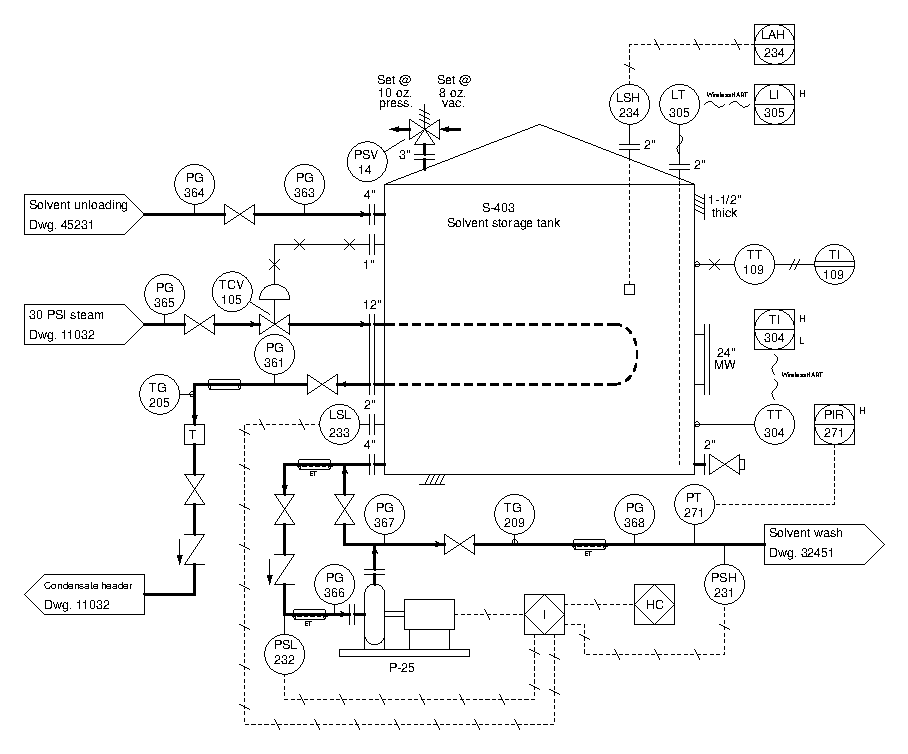
\includegraphics[width=15.5cm]{i0006rx01.eps}$$

Anta damptrykk PG-365 = 30 PSIG, mettet damp. Kondensat ut er 145 $^{o}$F (TG-205). PG-361 viser atmosfærisk trykk (0 PSIG) i kondensatlinjen.

Ved dampflow 15 lb/h: beregn omtrent hvor lang tid det tar å varme et nytt batch løsemiddel fra 50 $^{o}$F til 105 $^{o}$F, hvis volumet er 4300 gallon, tetthet 57 lb/ft$^{3}$ og spesifikk varme 0.73. Se bort fra varmetap i isolasjon.

\underbar{file i00973}
%(END_QUESTION)





%(BEGIN_ANSWER)

Jeg viser ikke hele løsningen her, men oppgaven deles i:

\begin{itemize}
\item{} Finn nødvendig varme for temperaturøkning i løsemiddel
\item{} Finn varmeeffekt levert av damp ved gitt masseflow
\item{} Del \underbar{nødvendig varme} (BTU) på \underbar{varmeeffekt} (BTU/h) for å få \underbar{tid} (h)
\end{itemize}

Damptabell er mest praktisk for å bestemme varmeoverføring per pund damp.

%(END_ANSWER)





%(BEGIN_NOTES)

Løsningsforslag gir total oppvarmingstid på omtrent {\bf 82.85 timer}, med idealiseringer som neglisjerer varmetap og ventildrosling nær settpunkt.

%INDEX% Physics, heat and temperature: saturated steam pressure versus temperature
%INDEX% Physics, heat and temperature: steam table
%INDEX% Process: solvent storage tank (realistic P&ID shown)

%(END_NOTES)

